\chapter{Results}
\label{chap:results}
\sloppy

The results follow the analytical sequence established in the research questions. Instrument sensitivity is reported before persona composition and topology are interpreted. The D-net evidence then tests whether those patterns survive a change from generated eight-node graphs to the separate 63-node complex network.

% Drafted from thesisExperiment/analysis_full live outputs on 2026-09-19.
% Primary sources:
%   tables/c2_homo_t2c_vs_t2d_by_topology.csv
%   tables/c2_homo_t2c_vs_t2d_paired_live_cells.csv
%   tables/c3_hetero_t2c_vs_t2d_by_topology.csv
%   tables/c3_hetero_t2c_vs_t2d_paired_live_cells.csv
%   tables/c4_cross_mode_by_topology.csv
%   tables/ifd_dual_agreement_gap.csv
%   key_numbers.json

\section{Results: MPR instrument contrasts}
\label{sec:results-mpr}

This section compares the continuous-only campaign (T2c) with the
dual campaign's discrete headline (T2d).  The comparison is between
instruments, not between two estimates on a common ground-truth scale.
For each scored event, the discrete instrument counts the five audit items
classified as missing or incorrect and therefore returns an integer from
0 to 5.  The continuous instrument combines graded item scores into a
floating-point value on approximately the same range.  In a dual run, the
discrete value is the headline; the continuous value produced for the same
event is retained only as a sidecar diagnostic.

All results below are descriptive point estimates from one campaign
replicate and eight hops.  Dead cells are excluded from means and are never
replaced by zero.  ``Paired'' denotes a shared topology--persona/mix--article
cell that was live in both separately run campaigns; it does not turn the
two auditor outputs into repeated measurements by a single instrument.

\subsection{C2: homogeneous arm, different instruments}
\label{subsec:c2-mpr}

Holding the homogeneous arm fixed, T2d is higher than T2c on all eight
topologies (\cref{tab:c2c3-mpr}).  Averaging the eight topology-specific
differences gives
\[
  \overline{\Delta}_{\mathrm{H}}
  = \overline{\mathrm{T2d_H}-\mathrm{T2c_H}}
  = 0.8201346884 .
\]
The differences range from 0.6999 on the linear chain to 0.9494 in the
echo chamber.  There are 398 cells live in both campaigns.  Their median
paired difference is 0.8125; 342 differences are positive, 26 are negative,
and 30 are zero.  A further 80 cells are dead only in T2c, 82 only in T2d,
and 16 in both, so none of these cells enters the paired difference.

\begin{table}[t]
\centering
\caption{C2 and C3 live-cell headline means by topology.  Each
$\Delta$ is dual-discrete minus continuous within the stated arm.  Values
are reported to four decimal places from the live full-analysis tables.}
\label{tab:c2c3-mpr}
\small
\begin{tabular}{lrrrrrr}
\toprule
Topology
  & T2c H & T2d H & $\Delta_{\mathrm{H}}$
  & T2c He & T2d He & $\Delta_{\mathrm{He}}$ \\
\midrule
Linear chain & 0.9129 & 1.6127 & 0.6999 & 0.8638 & 2.0852 & 1.2214 \\
Ring         & 0.9160 & 1.6402 & 0.7242 & 0.8760 & 2.1768 & 1.3008 \\
Random ER    & 0.8736 & 1.7809 & 0.9073 & 0.6593 & 2.0412 & 1.3818 \\
Small world  & 0.7215 & 1.5977 & 0.8762 & 0.7545 & 1.9096 & 1.1552 \\
Scale-free   & 0.9205 & 1.7034 & 0.7829 & 0.8157 & 1.9924 & 1.1767 \\
Echo chamber & 0.8490 & 1.7984 & 0.9494 & 1.3775 & 1.9632 & 0.5857 \\
Polarised    & 0.8356 & 1.7005 & 0.8649 & 1.4137 & 1.8830 & 0.4693 \\
Hierarchical & 0.8751 & 1.6315 & 0.7564 & 1.5242 & 2.5934 & 1.0692 \\
\midrule
Mean topology $\Delta$
  & \multicolumn{2}{r}{} & 0.8201
  & \multicolumn{2}{r}{} & 1.0450 \\
\bottomrule
\end{tabular}
\end{table}

The dual-run diagnostics locate this separation inside the scoring
procedure.  On the same dual events, the mean absolute gap between the
discrete headline and its continuous sidecar is 0.8804 in H, while mean
agreement is 0.6487.  Agreement is the Pearson correlation between the
item-level continuous scores and discrete responses mapped from
$\{-1,0,+1\}$ to $\{0,0.5,1\}$.  It is therefore a within-event scoring
diagnostic, not accuracy against external labels.  Likewise, the absolute
dual gap is not a third MPR and the sidecar is not the separately generated
T2c headline.

\subsection{C3: heterogeneous arm, different instruments}
\label{subsec:c3-mpr}

The heterogeneous arm shows the same directional instrument separation:
T2d is above T2c on all eight topologies.  The topology-equal difference is
\[
  \overline{\Delta}_{\mathrm{He}}
  = \overline{\mathrm{T2d_{He}}-\mathrm{T2c_{He}}}
  = 1.0450048645 .
\]
The topology differences range from 0.4693 on the polarised graph to
1.3818 on random ER.  Of the 198 cells live in both campaigns, the median
paired difference is 0.97785; 169 differences are positive, 25 are negative,
and 4 are zero.  Cells dead on one side are again excluded: 42 are dead only
in T2c, 40 only in T2d, and 8 in both.

Within the He dual runs, the same-event mean absolute dual gap is 1.1145
and mean agreement is 0.6174.  The gap is larger and agreement lower than
their H summaries, but these are descriptive diagnostics; with one
replicate they do not establish an arm effect.  The live tables do not
contain CR, MR, IR, or hop-level MI, so no corresponding contrasts are
reported.

\begin{table}[t]
\centering
\caption{Same-event dual diagnostics by topology.  Gap is the mean
absolute difference between the discrete headline and continuous sidecar;
agreement is their item-level response correlation.  Neither column is an
additional MPR.}
\label{tab:mpr-diagnostics}
\small
\begin{tabular}{lrrrr}
\toprule
Topology & H gap & H agreement & He gap & He agreement \\
\midrule
Linear chain & 0.9672 & 0.6223 & 1.2960 & 0.7196 \\
Ring         & 0.8803 & 0.6656 & 1.3123 & 0.6404 \\
Random ER    & 0.9680 & 0.6969 & 1.1335 & 0.6460 \\
Small world  & 0.8255 & 0.5928 & 1.1049 & 0.6522 \\
Scale-free   & 0.8463 & 0.6607 & 1.1058 & 0.6230 \\
Echo chamber & 0.8923 & 0.6306 & 0.8830 & 0.5986 \\
Polarised    & 0.8553 & 0.6191 & 0.8784 & 0.5673 \\
Hierarchical & 0.7973 & 0.6906 & 1.1354 & 0.2947 \\
\midrule
Live-cell summary & 0.8804 & 0.6487 & 1.1145 & 0.6174 \\
\bottomrule
\end{tabular}
\end{table}

\subsection{Why level and rank need not agree}
\label{subsec:mpr-ranks}

The consistent level ordering does not imply a consistent topology ranking.
In H, the topology-mean rank correlation between continuous and discrete
headlines is $\rho=0.0952$; in He it is $\rho=0.1667$ (eight topology means
in each arm).  These coefficients are descriptive and are not used as
inferential tests.

The apparent combination---T2d above T2c everywhere, but weak agreement in
rank---follows from two distinct comparisons.  The first asks whether the
discrete level exceeds the continuous level within each topology.  The
second asks whether the size ordering among topologies is preserved.  It is
not: the instrument increment is topology-dependent rather than a constant
offset.  For example, the H increment is 0.6999 on the linear chain but
0.9494 in the echo chamber; in He it is 0.4693 on the polarised graph but
1.3818 on random ER.  The instruments also use different response
representations---hard missing/incorrect counts versus graded scores---and
the T2c and T2d campaigns make separate auditor calls.  Thus borderline
item judgements can change both scale spacing and rank.

These observations explain why ``discrete is higher'' is an instrument
result, not evidence that discrete scoring recovered more true
misinformation.  Continuous scoring is not a ground-truth benchmark for
discrete scoring, and discrete scoring is not a ground-truth correction of
continuous scoring.  The same-event gaps and non-unit agreement document
their divergence; they do not adjudicate which instrument is more valid.

\subsection{C4: cross-mode, two-factor contrast}
\label{subsec:c4-mpr}

C4 changes arm and instrument simultaneously.  Comparing T2d He with T2c H
gives a positive mean topology difference,
\[
  \overline{\mathrm{T2d_{He}}-\mathrm{T2c_H}}
  = 1.2175517040 ,
\]
whereas comparing T2c He with T2d H gives
\[
  \overline{\mathrm{T2c_{He}}-\mathrm{T2d_H}}
  = -0.6475878488 .
\]
The sign reverses on every topology when the instrument is swapped against
the arm (\cref{tab:c4-mpr}).  This is expected given the large
instrument-level separation in C2 and C3.  It prevents either cross-mode
difference from being interpreted as an H--He effect: each combines
identity composition and scoring mode, and neither factor is held fixed.

\begin{table}[t]
\centering
\caption{C4 cross-mode topology means and exact contrast direction.
The two deltas change arm and instrument together and are not averaged into
a headline.}
\label{tab:c4-mpr}
\small
\begin{tabular}{lrrrrrr}
\toprule
Topology
  & T2c H & T2d He & $\Delta(\mathrm{T2d_{He}}-\mathrm{T2c_H})$
  & T2d H & T2c He & $\Delta(\mathrm{T2c_{He}}-\mathrm{T2d_H})$ \\
\midrule
Linear chain & 0.9129 & 2.0852 & 1.1724 & 1.6127 & 0.8638 & $-0.7489$ \\
Ring         & 0.9160 & 2.1768 & 1.2608 & 1.6402 & 0.8760 & $-0.7642$ \\
Random ER    & 0.8736 & 2.0412 & 1.1675 & 1.7809 & 0.6593 & $-1.1216$ \\
Small world  & 0.7215 & 1.9096 & 1.1881 & 1.5977 & 0.7545 & $-0.8432$ \\
Scale-free   & 0.9205 & 1.9924 & 1.0719 & 1.7034 & 0.8157 & $-0.8877$ \\
Echo chamber & 0.8490 & 1.9632 & 1.1141 & 1.7984 & 1.3775 & $-0.4209$ \\
Polarised    & 0.8356 & 1.8830 & 1.0474 & 1.7005 & 1.4137 & $-0.2868$ \\
Hierarchical & 0.8751 & 2.5934 & 1.7182 & 1.6315 & 1.5242 & $-0.1074$ \\
\midrule
Mean topology $\Delta$
  & \multicolumn{2}{r}{} & 1.2176
  & \multicolumn{2}{r}{} & $-0.6476$ \\
\bottomrule
\end{tabular}
\end{table}

Accordingly, C4 remains a labelled sensitivity contrast.  Averaging its two
deltas would cancel differences created by swapping instruments and would
produce a quantity with no instrument-specific interpretation.  No pooled
C4 MPR is therefore reported.


\section{Persona composition, article valence, and cascade persistence}
\label{sec:results-personas}

This section separates the homogeneous-persona (\textbf{H}) and heterogeneous-mix
(\textbf{He}) arms before interpreting them.  The labels describe how identities
were assigned to the eight nodes: every node received the same persona in H,
whereas He used a documented mixture of eight persona identifiers.  They do not
denote low- and high-diversity treatments with otherwise matched content.
In particular, the H arm pools conspiracy personas with climate-action and
science/environment personas, while the He arm pools conspiracy-heavy,
conspiracy-sparse, and conspiracy-free compositions.  Consequently, an
aggregate H--He difference combines composition with heterogeneity and cannot
by itself identify an effect of diversity.

\subsection{Homogeneous persona families}

Figures~10--12 cross the twelve H personas with the six articles.  Figure~10
shows mean misinformation persistence rate (MPR), Figure~11 shows maximum
misinformation intensity (MI), and Figure~12 shows the irreversible crossing
time \(k^*\).  The columns in these heatmaps are not replicates: each cell is
one seed, and dead cells are excluded rather than entered as zero.

The strongest separation is by persona family.  Across live H cells, the four
conspiracy personas have continuous MPR \(2.2194\) (\(168\) live cells) and
dual-discrete MPR \(3.1691\) (\(159\) live cells).  Their \(k^*\) rates are
\(40.5\%\) and \(59.7\%\), respectively.  Climate-action personas are much
lower: continuous MPR \(0.1729\) (\(117\) live) and dual-discrete MPR \(1.0488\)
(\(126\) live), with \(k^*\) rates \(0.0\%\) and \(0.8\%\).  The
science/environment family is lowest on continuous MPR, \(0.1118\) (\(195\)
live), but its dual-discrete MPR, \(0.8687\) (\(193\) live), is not zero; its
\(k^*\) rate is \(0.0\%\) in both instruments.  Thus the discrete instrument
can assign nonzero persistence to science/environment personas without those
runs ever locking above the \(k^*\) threshold.  Figure~20 supports reading
this as instrument disagreement: across all live H dual cells the mean
discrete-minus-sidecar-continuous gap is \(0.8804\), and mean agreement is
\(0.6487\).

\begin{table}[t]
\centering
\caption{Homogeneous personas, collapsed across eight topologies and six
articles.  MPR means and \(k^*\) rates use live cells only; each persona has 48
expected cells per instrument.}
\label{tab:results-personas}
\scriptsize
\begin{tabular}{llrrrrrrrr}
\toprule
Persona & Family & \(n_c\) & MPR\(_c\) & \(k^*_c\) &
\(n_d\) & MPR\(_d\) & \(k^*_d\) & Dead \(c/d\) \\
\midrule
conspiracy\_believer & conspiracy & 44 & 2.4842 & 47.7\% & 38 & 3.3522 & 65.8\% & 4/10 \\
conspiracy\_haarp\_weather & conspiracy & 40 & 2.4829 & 47.5\% & 44 & 3.3571 & 70.5\% & 8/4 \\
conspiracy\_depopulation & conspiracy & 43 & 1.9535 & 34.9\% & 37 & 3.2823 & 59.5\% & 5/11 \\
conspiracy\_climate\_piggyback & conspiracy & 41 & 1.9570 & 31.7\% & 40 & 2.6838 & 42.5\% & 7/8 \\
climate\_action\_advocate & climate action & 37 & 0.2258 & 0.0\% & 37 & 1.0665 & 0.0\% & 11/11 \\
climate\_justice\_youth & climate action & 41 & 0.2454 & 0.0\% & 46 & 1.3072 & 2.2\% & 7/2 \\
mitigation\_first\_policy & climate action & 39 & 0.0464 & 0.0\% & 43 & 0.7571 & 0.0\% & 9/5 \\
environmental\_concern & science/env. & 40 & 0.1423 & 0.0\% & 37 & 0.8359 & 0.0\% & 8/11 \\
biodiversity\_food\_security & science/env. & 39 & 0.2115 & 0.0\% & 37 & 1.1470 & 0.0\% & 9/11 \\
ozone\_stratosphere\_specialist & science/env. & 38 & 0.1627 & 0.0\% & 37 & 0.9639 & 0.0\% & 10/11 \\
science\_journalist & science/env. & 37 & 0.0310 & 0.0\% & 39 & 0.6745 & 0.0\% & 11/9 \\
climate\_scientist & science/env. & 41 & 0.0130 & 0.0\% & 43 & 0.7517 & 0.0\% & 7/5 \\
\bottomrule
\end{tabular}
\end{table}

The individual rows qualify the family averages.  On continuous MPR,
\texttt{conspiracy\_believer} (\(2.4842\)) and
\texttt{conspiracy\_haarp\_weather} (\(2.4829\)) are nearly tied, whereas
\texttt{conspiracy\_depopulation} (\(1.9535\)) and
\texttt{conspiracy\_climate\_piggyback} (\(1.9570\)) form a lower pair.  The
dual-discrete ordering changes: \texttt{conspiracy\_haarp\_weather} is highest
at \(3.3571\), followed by \texttt{conspiracy\_believer} at \(3.3522\),
\texttt{conspiracy\_depopulation} at \(3.2823\), and
\texttt{conspiracy\_climate\_piggyback} at \(2.6838\).  Their dual \(k^*\)
rates span \(42.5\%\)--\(70.5\%\); the corresponding continuous range is
\(31.7\%\)--\(47.7\%\).

Among the climate-action personas, \texttt{climate\_justice\_youth} is highest
on both instruments (continuous \(0.2454\), dual \(1.3072\)); it is also the
only non-conspiracy H persona with any observed \(k^*\), a \(2.2\%\) dual rate
(one of 46 live cells).  \texttt{mitigation\_first\_policy} is lowest in that
family (continuous \(0.0464\), dual \(0.7571\)).  Within science/environment,
\texttt{biodiversity\_food\_security} is highest (continuous \(0.2115\), dual
\(1.1470\)), while \texttt{climate\_scientist} has the lowest continuous MPR
(\(0.0130\)) and \texttt{science\_journalist} the lowest dual MPR (\(0.6745\)).
These differences are visible by article in Figures~10 and~12 and by topology
in Figure~15.  Figure~11 is also important methodologically: maximum MI can be
high when average persistence is modest, so a transient peak should not be
reported as a sustained firestorm.

\subsection{Heterogeneous compositions}

Figures~13 and~14 provide the corresponding mix-by-article heatmaps for mean
MPR and maximum MI, and Figure~16 crosses each mix with topology.  The
conspiracy content of the mix tracks the principal MPR gradient more closely
than the generic He label.  The most direct contrast is between
\texttt{mix\_00} (four conspiracy plus four climate/environment personas) and
\texttt{mix\_02} (zero conspiracy plus eight science/climate personas).
\texttt{mix\_00} reaches continuous MPR \(1.7712\) and dual-discrete MPR
\(3.1321\), compared with \(0.2645\) and \(1.1882\) for \texttt{mix\_02}.
Its \(k^*\) rates are \(12.8\%\) continuous and \(57.5\%\) dual, whereas
\texttt{mix\_02} is \(0.0\%\) on both.

\begin{table}[t]
\centering
\caption{Heterogeneous mixes collapsed across topologies and articles.  Counts
and \(k^*\) rates refer to live cells; each mix has 48 expected cells per
instrument.}
\label{tab:results-mixes}
\scriptsize
\begin{tabular}{llrrrrrrrr}
\toprule
Mix & Composition & \(n_c\) & MPR\(_c\) & \(k^*_c\) &
\(n_d\) & MPR\(_d\) & \(k^*_d\) & Dead \(c/d\) \\
\midrule
mix\_00 & 4 conspiracy + 4 climate/env. & 39 & 1.7712 & 12.8\% & 40 & 3.1321 & 57.5\% & 9/8 \\
mix\_01 & 2 conspiracy + 6 climate/env. & 41 & 1.4770 & 9.8\% & 41 & 2.7795 & 58.5\% & 7/7 \\
mix\_02 & 0 conspiracy + 8 science/climate & 41 & 0.2645 & 0.0\% & 41 & 1.1882 & 0.0\% & 7/7 \\
mix\_03 & 1 conspiracy + 7 other & 39 & 0.8945 & 10.3\% & 36 & 2.0410 & 33.3\% & 9/12 \\
mix\_04 & 2 conspiracy-adj. + 6 other & 38 & 0.7021 & 5.3\% & 39 & 1.6896 & 20.5\% & 10/9 \\
mix\_05 & 2 conspiracy-adj. + 6 other & 40 & 1.0134 & 7.5\% & 43 & 1.6713 & 23.3\% & 8/5 \\
\bottomrule
\end{tabular}
\end{table}

\texttt{mix\_01}, with two conspiracy personas, remains high (continuous
\(1.4770\), dual \(2.7795\)) and has the highest dual \(k^*\) rate,
\(58.5\%\).  A single conspiracy persona in \texttt{mix\_03} is associated
with MPR \(0.8945\) continuous and \(2.0410\) dual, with \(k^*\) rates
\(10.3\%\) and \(33.3\%\).  The two conspiracy-adjacent compositions do not
produce a monotone dose response: \texttt{mix\_04} is lower than
\texttt{mix\_05} continuously (\(0.7021\) versus \(1.0134\)), but slightly
higher in dual-discrete scoring (\(1.6896\) versus \(1.6713\)).  Nor is
\texttt{mix\_00} uniformly above \texttt{mix\_01}: its MPR is higher, but its
dual \(k^*\) rate is lower by \(1.0\) percentage point.  The defensible result
is therefore compositional---conspiracy-heavy mixes generally score above the
conspiracy-free mix---rather than a universal claim that heterogeneous
networks amplify or suppress a cascade.

\subsection{Article valence and topology}

Article effects cut across persona composition.  Figures~21 and~22 collapse
the six articles separately for H and He, while Figure~17 shows the
topology-by-article pattern.  The exact article means are:

\begin{table}[t]
\centering
\caption{Article-level live-cell MPR by arm and instrument.}
\label{tab:results-articles}
\scriptsize
\begin{tabular}{lrrrr}
\toprule
Article & H continuous & H dual & He continuous & He dual \\
\midrule
\texttt{scopex\_2017} & 0.7322 & 1.5390 & 0.7694 & 2.3718 \\
\texttt{chemtrails\_gates\_2018\_2021} & 1.3541 & 2.1383 & 1.7852 & 2.3885 \\
\texttt{sai\_geoengineering} & 0.1974 & 1.3576 & 0.1523 & 1.1160 \\
\texttt{paris\_agreement} & 1.3357 & 1.7321 & 1.6821 & 2.4591 \\
\texttt{climate\_consensus} & 1.5934 & 2.2610 & 1.8896 & 2.8991 \\
\texttt{polar\_bears} & 0.0185 & 1.0399 & 0.0415 & 1.1444 \\
\bottomrule
\end{tabular}
\end{table}

\texttt{climate\_consensus} is highest in all four arm--instrument
combinations: H continuous \(1.5934\), H dual \(2.2610\), He continuous
\(1.8896\), and He dual \(2.8991\).  \texttt{polar\_bears} is lowest in all
four (\(0.0185\), \(1.0399\), \(0.0415\), and \(1.1444\), respectively).
The chemtrails--Gates article is consistently above SCoPEx: \(1.3541\) versus
\(0.7322\) in H continuous, \(2.1383\) versus \(1.5390\) in H dual,
\(1.7852\) versus \(0.7694\) in He continuous, and \(2.3885\) versus
\(2.3718\) in He dual.  However, ``valence'' bundles topic, framing, and fit
with a persona's prior narrative.  Figures~10 and~13 show that it is an
interaction, not an article-only treatment.

\subsection{\texorpdfstring{\(k^*\)}{k-star} and dead-cell sensitivity}

Figure~19 summarizes irreversible crossings over eight ticks.  Collapsed H
\(k^*\) rates are \(14.2\%\) continuous and \(20.1\%\) dual; collapsed He
rates are \(7.6\%\) and \(32.1\%\).  The reversed continuous/dual H--He
ordering is further evidence against assigning a single causal meaning to the
arm label.  It also shows why \(k^*\) should not be inferred from MPR alone:
the dual He arm has both a much higher crossing rate and a different scoring
scale.  With only eight ticks, ``no \(k^*\)'' means no observed irreversible
crossing within the window, not proof that a later crossing is impossible.

Figure~18 reports the missingness generated after real LLM calls.  Of 1,728
expected thesis cells, 292 are dead (\texttt{nScored}\(\leq 1\)); they remain
hatched and are never converted to zeros.  By arm and instrument, dead rates
are \(16.7\%\) for H continuous (480/576 live), \(17.4\%\) for He continuous
(238/288 live), \(17.0\%\) for H dual (478/576 live), and \(16.7\%\) for He
dual (240/288 live).  Missingness is not uniform by topology.  The largest
rate is polarised He continuous at \(30.6\%\) (25/36 live), followed by
hierarchical H continuous and hierarchical He continuous, both \(27.8\%\)
(52/72 and 26/36 live), and polarised He dual at \(27.8\%\) (26/36 live).
At the low end, linear-chain H dual is \(5.6\%\) dead (68/72 live), and ring
He is \(8.3\%\) dead in both instruments (33/36 live).

Accordingly, the means in Figures~10--17 and~21--22 describe surviving scored
cascades.  The dead-rate pattern is part of the result: a pale heatmap cell
means low MPR among live runs, while a hatched cell supplies no MPR estimate.
Neither dead He cells nor the \(0.0\%\) \(k^*\) rate of \texttt{mix\_02}
demonstrates that heterogeneous or expert-inclusive networks are immune.
Together, Figures~10--22 support a narrower conclusion: persona and article
composition strongly structure observed persistence, the dual instrument
usually scores higher and crosses \(k^*\) more often, and topology-dependent
dead cells limit causal interpretation of the H/He contrast.


% Draft results section: topology and same-mode H--He comparison (C1).
% Sources: analysis_full/COMPARISONS.md, key_numbers.json, and
% tables/c1_same_mode_h_vs_he_by_topology.csv.

\section{Topology results}
\label{sec:results-topology}

This section reports the eight-topology sweep and comparison C1, which holds
the scoring mode fixed while comparing homogeneous (H) and heterogeneous (He)
identity assignments.  The harvest contains one graph seed
(\texttt{graphRandomSeed=42}; $N=1$), so all differences below are descriptive
properties of these runs.  They do not identify a causal effect of topology or
identity composition.

There were 72 candidate H cells per topology and mode (12 personas $\times$ 6
articles) and 36 candidate He cells (6 mixes $\times$ 6 articles).  A cell was
classified as dead when \texttt{nScored}$\leq 1$ after the LLM calls.  Dead
cells were retained and hatched in the grids, but were neither replaced by
zero nor included in the means.  Thus, the denominators in
\Cref{tab:topology-continuous,tab:topology-dual} vary by topology.  Across the
full $1{,}728$-cell harvest, 292 cells were dead (rather than the preliminary
brief's 290).

\subsection{Continuous instrument}
\label{sec:results-topology-continuous}

\Cref{tab:topology-continuous} reports the continuous-only (T2c) headline
separately from the dual-discrete results.  Among H cells, the topology means
ranged from 0.7215 for small world ($56/72$ live) to 0.9205 for scale-free
($60/72$ live).  Among He cells, they ranged from 0.6593 for random ER
($29/36$ live) to 1.5242 for hierarchical ($26/36$ live).  These extrema
describe live cells only; for example, hierarchical He had 10 dead cells and
polarised He had 11.

\begin{table}[t]
\centering
\caption{Continuous (T2c) live-cell mean \texttt{meanMI} by topology and C1
same-mode difference.  ``Live'' gives the scored numerator and full-cell
denominator; dead is the excluded-from-mean count.  $\Delta=\mathrm{He}-\mathrm{H}$.
$N=1$.}
\label{tab:topology-continuous}
\scriptsize
\begin{tabular}{lrrrrrrr}
\toprule
Topology & H live & H dead & H mean & He live & He dead & He mean & $\Delta$ \\
\midrule
linear chain & 62/72 & 10 & 0.9129 & 32/36 & 4  & 0.8638 & $-0.0491$ \\
ring         & 65/72 & 7  & 0.9160 & 33/36 & 3  & 0.8760 & $-0.0400$ \\
random ER    & 57/72 & 15 & 0.8736 & 29/36 & 7  & 0.6593 & $-0.2143$ \\
small world  & 56/72 & 16 & 0.7215 & 31/36 & 5  & 0.7545 & $\phantom{-}0.0330$ \\
scale-free   & 60/72 & 12 & 0.9205 & 30/36 & 6  & 0.8157 & $-0.1048$ \\
echo chamber & 63/72 & 9  & 0.8490 & 32/36 & 4  & 1.3775 & $\phantom{-}0.5284$ \\
polarised    & 65/72 & 7  & 0.8356 & 25/36 & 11 & 1.4137 & $\phantom{-}0.5780$ \\
hierarchical & 52/72 & 20 & 0.8751 & 26/36 & 10 & 1.5242 & $\phantom{-}0.6490$ \\
\bottomrule
\end{tabular}
\end{table}

The continuous C1 sign was not uniform.  He exceeded H on four of eight
topologies (small world, echo chamber, polarised, and hierarchical), whereas H
exceeded He on linear chain, ring, random ER, and scale-free.  Giving each
topology equal weight, the mean $\Delta(\mathrm{He}-\mathrm{H})$ was 0.1725.
Pooling live cells instead gave H 0.8643 ($n=480/576$ live) and He 1.0192
($n=238/288$ live), a difference of 0.1549.  The two summaries differ because
live-cell counts vary; neither treats the 146 dead continuous cells as zeros.

The near-balanced signs are visible in the continuous panel of
\Cref{fig:c1-h-he,fig:c1-delta}.  An exploratory signed-rank summary of the
eight topology means was $W=14$, $p=0.6406$, with median delta $-0.0035$
($n_{+}=4$, $n_{-}=4$).  These eight means come from one seed and are not
independent experimental replicates; the calculation is therefore a compact
description, not replicate-level inference.

\subsection{Dual-discrete instrument}
\label{sec:results-topology-dual}

\Cref{tab:topology-dual} reports the discrete headline from dual runs (T2d).
It is a different instrument from T2c and is not averaged with the continuous
headline.  H means ranged from 1.5977 for small world ($59/72$ live) to 1.7984
for echo chamber ($61/72$ live).  He means ranged from 1.8830 for polarised
($26/36$ live) to 2.5934 for hierarchical ($28/36$ live).

\begin{table}[t]
\centering
\caption{Dual-discrete (T2d) live-cell mean \texttt{meanMI} by topology and C1
same-mode difference.  ``Live'' gives the scored numerator and full-cell
denominator; dead is the excluded-from-mean count.  $\Delta=\mathrm{He}-\mathrm{H}$.
$N=1$.}
\label{tab:topology-dual}
\scriptsize
\begin{tabular}{lrrrrrrr}
\toprule
Topology & H live & H dead & H mean & He live & He dead & He mean & $\Delta$ \\
\midrule
linear chain & 68/72 & 4  & 1.6127 & 33/36 & 3  & 2.0852 & 0.4725 \\
ring         & 61/72 & 11 & 1.6402 & 33/36 & 3  & 2.1768 & 0.5366 \\
random ER    & 56/72 & 16 & 1.7809 & 29/36 & 7  & 2.0412 & 0.2602 \\
small world  & 59/72 & 13 & 1.5977 & 32/36 & 4  & 1.9096 & 0.3120 \\
scale-free   & 57/72 & 15 & 1.7034 & 29/36 & 7  & 1.9924 & 0.2890 \\
echo chamber & 61/72 & 11 & 1.7984 & 30/36 & 6  & 1.9632 & 0.1647 \\
polarised    & 57/72 & 15 & 1.7005 & 26/36 & 10 & 1.8830 & 0.1825 \\
hierarchical & 59/72 & 13 & 1.6315 & 28/36 & 8  & 2.5934 & 0.9618 \\
\bottomrule
\end{tabular}
\end{table}

He exceeded H on all eight dual-discrete topology means.  The topology-equal
mean difference was 0.3974.  Pooling live cells gave H 1.6814
($n=478/576$ live) and He 2.0800 ($n=240/288$ live), a difference of 0.3986;
the 146 dead dual cells were not imputed.  The largest topology-level gap was
hierarchical (0.9618), and the smallest was echo chamber (0.1647).

For completeness, the exploratory signed-rank summary across the eight
topology means was $W=0$, $p=0.007812$, with median delta 0.3005
($n_{+}=8$, $n_{-}=0$).  Because $N=1$, this is not evidence of a general
identity-mix effect.  In particular, collapsed H combines conspiracy personas
with low-scoring scientist personas, while collapsed He combines
conspiracy-heavy and conspiracy-free mixes.  The observed ordering therefore
does not support a causal claim that heterogeneity increases or buffers
firestorms.

\begin{figure}[t]
\centering
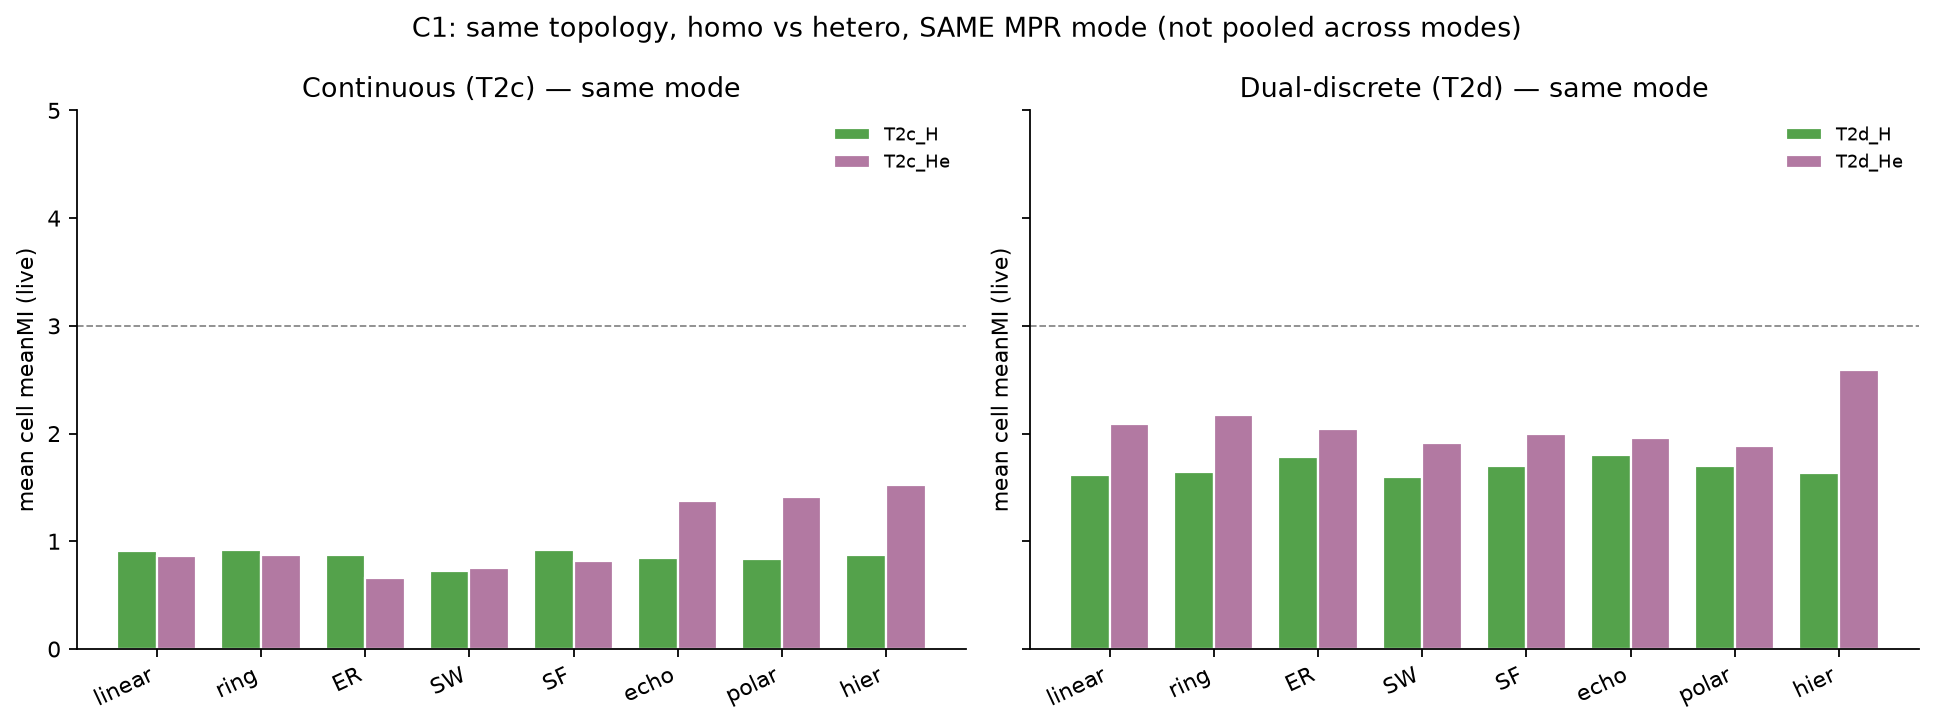
\includegraphics[width=\textwidth]{figures/fig01_c1_h_vs_he_same_mode.png}
\caption{C1 same-mode H and He live-cell means for all eight topologies.
Continuous and dual-discrete panels remain separate; dead cells are excluded
from means rather than set to zero.  $N=1$.}
\label{fig:c1-h-he}
\end{figure}

\begin{figure}[t]
\centering
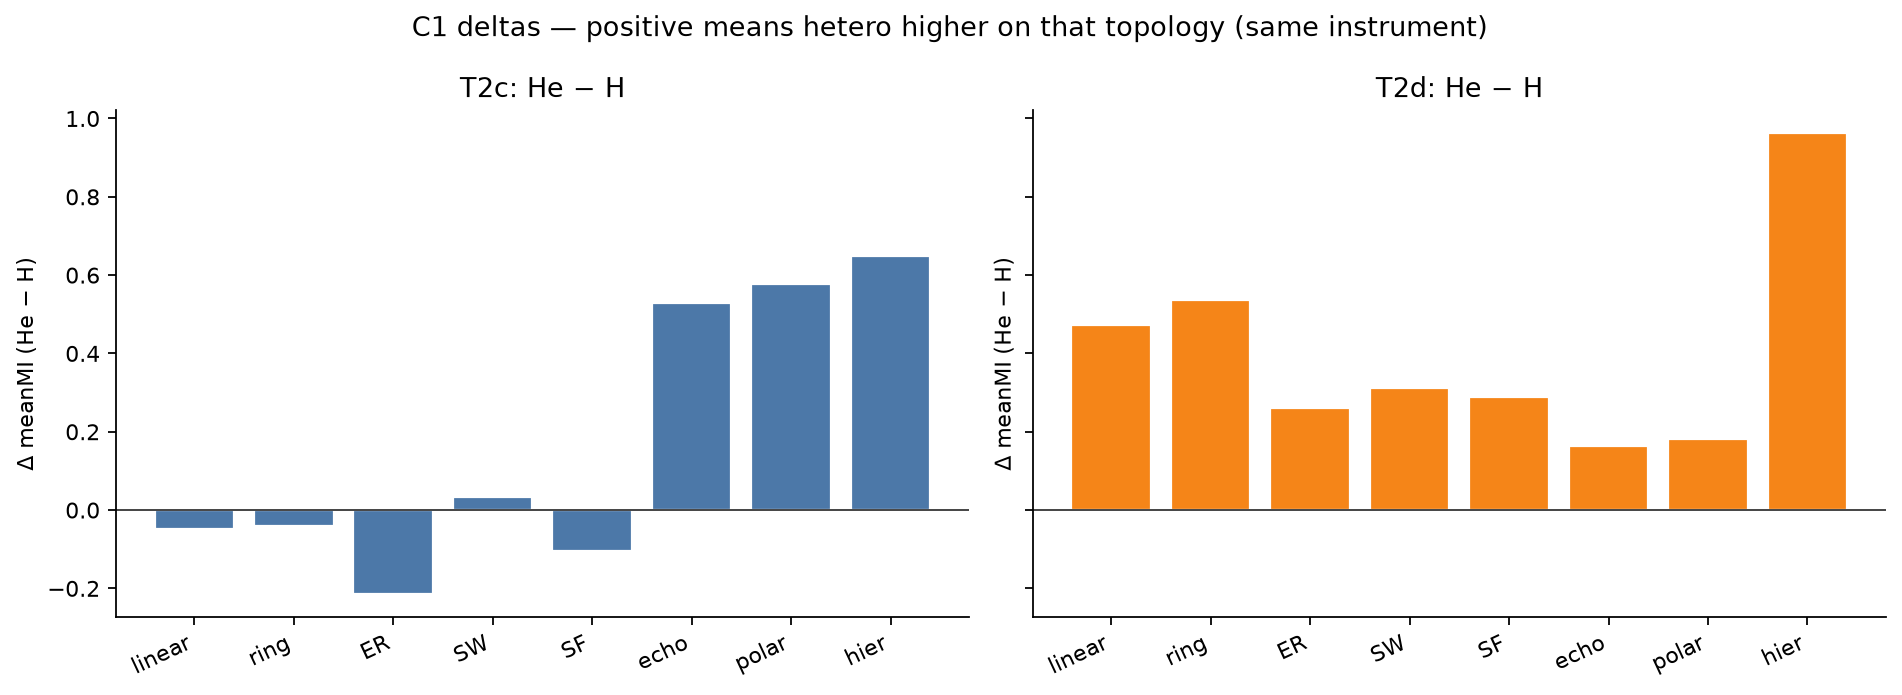
\includegraphics[width=\textwidth]{figures/fig02_c1_delta_he_minus_h.png}
\caption{C1 topology-level $\Delta(\mathrm{He}-\mathrm{H})$.  Continuous has
four positive and four negative differences; dual-discrete has eight positive
differences.  These are descriptive one-seed contrasts.}
\label{fig:c1-delta}
\end{figure}

The article-resolved topology pattern is shown in
\texttt{fig17\_topology\_article\_mpr.png}; topology-by-persona and
topology-by-mix views are in \texttt{fig15\_persona\_topology\_mpr.png} and
\texttt{fig16\_mix\_topology\_mpr.png}.  The corresponding denominators and
hatch pattern are visualised in \texttt{fig18\_dead\_rates.png}.  Those
figures should be read with the same live-only and mode-separation rules used
in the tables above.


\section{Results on the 63-node D-net}
\label{sec:results-dnet}

\subsection{Graph and persona placement}

The D-net experiments used the custom graph in
\path{thesisExperiment/data/derived/debnath_hashtag_cascade.json}.
It contains 63 nodes and 228 directed edges, collapsing to 171 unique
undirected pairs.  The nodes are accounts keyed by published hashtags and
the edges encode hashtag co-occurrence and same-cluster links.  Although the
edges occupy the importer's \texttt{retweets[]} field, they are not observed
retweets: Twitter/X hydration failed, and the object is not a retweet
cascade.  Both D-net persona conditions used exactly this topology and the
same seed node, \texttt{user\_chemtrails\_hub}.

The heterogeneous placement retained the reconstructed Debnath type mix.
Of the 63 placements, 56 used the exact reconstructed persona identifier.
The remaining seven used a coarser persona identifier while retaining the
mapped Debnath type:
\begin{itemize}
  \item \texttt{user\_depopulation\_amp}:
  \texttt{conspiracy\_depopulation} $\rightarrow$
  \texttt{conspiracy\_believer};
  \item \texttt{user\_climateaction\_piggyback\_amp} and
  \texttt{user\_climateaction\_piggyback\_peri\_1}:
  \texttt{conspiracy\_climate\_piggyback} $\rightarrow$
  \texttt{conspiracy\_believer};
  \item \texttt{user\_biodiversity\_hub},
  \texttt{user\_biodiversity\_peri\_1}, and
  \texttt{user\_foodsecurity\_amp}:
  \texttt{biodiversity\_food\_security} $\rightarrow$
  \texttt{environmental\_concern}; and
  \item \texttt{user\_mitigation\_amp}:
  \texttt{mitigation\_first\_policy} $\rightarrow$
  \texttt{climate\_action\_advocate}.
\end{itemize}
Thus the heterogeneous arm placed 28 conspiracy-family, 19
climate-action, 13 environmental, and three expert personas.  The
homogeneous arm instead assigned \texttt{conspiracy\_believer} to all 63
nodes.  The empirical hashtag identities were 28 conspiracy, 19
climate-action, 14 environmental-concern, and two other nodes; this
difference in counting reflects the coarser simulation placement, including
the type-only fallback for \texttt{user\_mitigation\_amp}, rather than a
change to the graph.

\subsection{Four D-net arms}

Four completed configurations crossed continuous versus dual-discrete
auditing with homogeneous conspiracy versus heterogeneous Debnath-mapped
personas.  Each configuration propagated two seed articles, producing the
eight article-level results in Table~\ref{tab:dnet-arms}.  These are
auditor scores from the simulation, not measurements made on Twitter.

\begin{table}[htbp]
\centering
\caption{Article-level auditor scores in the four D-net configurations.
The continuous sidecar from a dual run is shown only as a diagnostic and is
not interchangeable with the continuous-run headline.}
\label{tab:dnet-arms}
\small
\begin{tabular}{llrrr}
\toprule
Configuration & Article & Headline score & $n$ scored & Dual sidecar \\
\midrule
\texttt{Dnet\_c\_H\_conspiracy}
  & SCoPEx & 1.7349 & 970 & --- \\
\texttt{Dnet\_c\_H\_conspiracy}
  & chemtrails--Gates & 3.3378 & 984 & --- \\
\texttt{Dnet\_c\_He\_mixed}
  & SCoPEx & 0.9983 & 591 & --- \\
\texttt{Dnet\_c\_He\_mixed}
  & chemtrails--Gates & 2.5068 & 1,035 & --- \\
\texttt{Dnet\_d\_H\_conspiracy}
  & SCoPEx & 4.2537 & 1,076 & 2.2495 \\
\texttt{Dnet\_d\_H\_conspiracy}
  & chemtrails--Gates & 3.7303 & 749 & 3.1251 \\
\texttt{Dnet\_d\_He\_mixed}
  & SCoPEx & 2.6880 & 407 & 1.1302 \\
\texttt{Dnet\_d\_He\_mixed}
  & chemtrails--Gates & 1.5297 & 1,027 & 1.1497 \\
\bottomrule
\end{tabular}
\end{table}

Within each article and instrument, homogeneous conspiracy scored above the
mixed placement: 1.7349 versus 0.9983 and 3.3378 versus 2.5068 under the
continuous auditor, and 4.2537 versus 2.6880 and 3.7303 versus 1.5297 under
the dual-discrete auditor.  Article ordering depended on the instrument.
Chemtrails--Gates exceeded SCoPEx in both continuous arms, whereas SCoPEx
exceeded chemtrails--Gates in both dual-discrete arms.

\subsection{Do the small-topology findings hold?}

Only the composition result transfers cleanly.  In the eight-node grid,
conspiracy-family homogeneous cells were the high-score family on both
instruments (3.1691 dual-discrete and 2.2194 continuous).  The D-net result
is consistent with that finding: replacing the mixed type placement with
63 conspiracy-believer seats raised the score for both articles under both
auditors.

The collapsed H/He result does not transfer as an H/He law.  Across the
eight small topologies, collapsed He exceeded collapsed H by 0.1549 under
continuous scoring and by 0.3986 under dual-discrete scoring, although the
continuous He$>$H ordering held on only four of the eight individual
topologies.  On D-net, H exceeded He in all four like-for-like article and
instrument comparisons.  This reversal is consistent with the different
composition of the labels: small-topology H pooled conspiracy personas with
scientists, while D-net H means conspiracy-only.

Nor does the small-grid instrument ordering hold without exception.  The
eight-topology aggregates placed dual-discrete above continuous on every
topology.  On D-net, the dual headline exceeded the corresponding
continuous-run headline for homogeneous SCoPEx, homogeneous
chemtrails--Gates, and mixed SCoPEx, but not for mixed
chemtrails--Gates (1.5297 dual-discrete versus 2.5068 continuous).
Because these are different auditors, even the three concordant
comparisons are instrument differences rather than estimates in a shared
unit.  D-net has only one fixed 63-node topology, so it cannot replicate or
rank the eight small topology treatments.

\subsection{Auditor MI is not empirical Twitter MPR}

Debnath provides no empirical 0--5 misinformation-propagation-rate
(\textsc{mpr}) outcome for this graph.  The source tweet identifiers were
not hydrated, the graph has no empirical tweet clock, and no tweet-level
content score can be paired with a simulated event.  Accordingly, the
values in Table~\ref{tab:dnet-arms} are LLM-as-judge auditor misinformation
indices (\textsc{mi}) inside the simulation.  They must not be described as
Twitter \textsc{mpr}, as Twitter \textsc{mi}, or as a match to observed
misinformation.  The dual-discrete headline, its continuous sidecar, and
the continuous-only headline are also separate instruments and are not
averaged.

\subsection{Structural comparison and validation diagnostics}

The copied graph has global transitivity 0.3146, mean local clustering
0.5153, and mean unique degree 5.4286.  The
\texttt{user\_chemtrails\_hub} node has 33 unique neighbours.  Using
unweighted unique-undirected pairs, the mixed-label conspiracy cut has
Newman--Girvan modularity 0.4297; the homogeneous one-community partition
has modularity 0.  Mixed-label identity homophily is 0.8377
in the simulation; homogeneous identity homophily is 1.0 by construction,
so the latter is not evidence of an emergent echo chamber.

For the rooted cascade-shape comparison, the empirical object had depth
4, breadth 33, reached size 61, and structural virality 2.7.  Across 16
simulated D-net cascades, the corresponding means were 2.5625, 40.9375,
53.5, and 1.7963.  Breadth was the only one of the three validation metrics
(depth, breadth, and structural virality) within the pre-specified
30\% band; the resulting structural-similarity score was 0.6885.

The distributional diagnostics do not validate a digital twin.
With one empirical object and 16 simulated cascades, the
Kolmogorov--Smirnov results were $D=1.0000$, $p=0.1104$ for depth;
$D=0.8125$, $p=0.2954$ for breadth; and $D=1.0000$, $p=0.1104$ for
structural virality.  Jensen--Shannon divergence was 1.0000 for all three
metrics, and all three distribution-match flags were false.  The empirical
sample size of one makes the KS comparisons underpowered; their
non-significant $p$-values are not evidence of equivalence.  Finally, DTFS
was 0.2754, below the 0.70 validation threshold
(\texttt{isValidated=false}).  Its content-correlation component was fixed
at zero because no empirical \textsc{mpr} or tweet-text \textsc{mi} exists.
The structural evidence therefore supports a comparison of cascade shape,
not empirical misinformation fidelity or digital-twin validation.


\section{Applying the Pfeffer firestorm framework}
\label{sec:pfeffer-application}

\subsection{The original framework and the thesis remapping}

\Textcite{pfeffer2014firestorms} define an online firestorm as a sudden
discharge of large quantities of negative word-of-mouth and complaint
messages directed at a person, company, or group.  The messages are
predominantly opinion rather than fact and are therefore highly affective.
The article is a qualitative--synthetic account based on observed cases; it
does not present an agent-based model, a tipping-point estimator, or a
climate-discourse experiment.

The Outlook of \textcite{pfeffer2014firestorms} identifies seven
interrelated factors:
\begin{enumerate}
    \item \emph{speed and volume of communication};
    \item \emph{binary choices};
    \item \emph{network clusters};
    \item \emph{unrestrained information flow};
    \item \emph{lack of diversity};
    \item \emph{cross-media dynamics}; and
    \item \emph{network-triggered decision processes}.
\end{enumerate}
These are the original factors used here.  In particular, valence and
surprise are not numbered Outlook factors.  Valence is motivated by the
affective character in the paper's definition of a firestorm, while surprise
is a thesis operationalisation of the novelty, speed, and volume mechanism in
factor~1.

The thesis vocabulary---valence, surprise, identity, clustering, echo,
temporal, and cross-media---is consequently a computational remapping, not a
renaming of Pfeffer et al.'s list.  The first six terms describe variables or
observables that can at least partly be represented in the simulation;
cross-media is included as a seventh ledger row but is held because the model
has no legacy-media layer.  Conversely, Pfeffer et al.'s binary-choice factor
has no dedicated thesis row.  The agents choose among
\texttt{forward}, \texttt{reinterpret}, and \texttt{drop}, so the engine is
ternary rather than an implementation of the paper's like/share/retweet
either--or mechanism.

\begin{table}[t]
\centering
\caption{Original Outlook factors and their treatment in the thesis.  The
right-hand column is an operational mapping, not Pfeffer et al.'s
terminology.}
\label{tab:pfeffer-original-remap}
\small
\begin{tabular}{p{0.05\textwidth}p{0.32\textwidth}p{0.53\textwidth}}
\toprule
\# & Pfeffer et al.\ (2014) & Thesis treatment \\
\midrule
1 & Speed and volume of communication
  & Surprise (shock versus drip) and temporal horizon; surprise is held at
    drip and empirical timing is unavailable. \\
2 & Binary choices
  & No dedicated observable or sweep; simulated actions are ternary. \\
3 & Network clusters
  & Clustering and part of the echo measurement. \\
4 & Unrestrained information flow
  & Partly represented by echo and hub reach, but not the hundreds or
    thousands of weak ties discussed in the paper. \\
5 & Lack of diversity
  & Identity composition and part of echo/homophily; homogeneous versus
    mixed belief profiles are compared. \\
6 & Cross-media dynamics
  & Held; neither the empirical reconstruction nor the engine contains a
    legacy-media or newsroom layer. \\
7 & Network-triggered decision processes
  & Related to the temporal ledger row, but the four adoption stages are not
    logged or estimated. \\
\bottomrule
\end{tabular}
\end{table}

\subsection{Order of application: empirical structure before simulation}

The application proceeds in two distinct stages.  First, structural
observables are calculated on the empirical fallback derived from
\textcite{debnath2023conspiracy}.  This object is a hashtag co-occurrence
graph with 63 nodes, 228 directed edges, and 171 unique undirected pairs.
It is not a retweet, reply, follower, or \texttt{conversation\_id} cascade.
The 814,924 tweet identifiers in the associated dataset were not hydrated,
and the graph contains no usable tweet clock.  Its labels and edges can
therefore support a bounded comparison of hashtag structure, but not a
reconstruction of user-to-user diffusion.

Second, D-net imports the same 63-node, 228-edge topology and runs agents on
it.  This ordering matters: transitivity, local clustering, hub degree, and
the mixed-label conspiracy cut already exist before any simulated message is
generated.  D-net copies this structure; it does not produce or validate it.
The post-simulation evidence consists of content-auditor scores, realised
actions and reach on that fixed graph, together with label-dependent
quantities for the homogeneous and mixed assignments.

\paragraph{Empirical hashtag structure.}
The graph has global transitivity \(0.315\), mean local clustering \(0.515\),
and mean unique degree \(5.43\).  The \texttt{\#chemtrails} hub has 33 unique
neighbours.  On the 171 unique-undirected pairs, the six assigned graph
clusters have \(Q=0.5489\), the four assigned discourse identities have
\(Q=0.5322\), and the binary conspiracy cut has \(Q=0.4297\).
These label-partition statistics are distinct from clustering coefficients.
Identity edge homophily is \(0.873\);
belief-profile-family homophily is \(0.838\).  The identity composition is
28 conspiracy, 19 climate-action, 14 environmental, and two expert/other
nodes.  Thus conspiracy discourse is a plurality (\(28/63=0.444\)), not a
monoculture.

\paragraph{D-net after simulation.}
The mixed D-net condition retains 28 conspiracy nodes and the empirical
type-level composition, with 19 climate-action, 13 environmental, and three
expert nodes after belief-profile assignment.  The homogeneous condition
instead assigns all 63 seats the
\texttt{conspiracy\_believer} profile.  Because both conditions use the same
edge set, transitivity, local clustering, and hub degree remain \(0.315\),
\(0.515\), and 33.  Mixed D-net identity homophily is \(0.838\), whereas the
homogeneous value is \(1.0\) by construction.  The latter is not evidence
that an echo chamber emerged.  It is the mechanical result of giving every
node the same identity.  Mixed belief-profile families have \(Q=0.4908\),
and the mixed binary conspiracy cut has \(Q=0.4297\).  Under homogeneous
labels there is only one community, for which \(Q=0\).

Across the four primary D-net cells, 61 of 63 nodes receive a message within
the held eight-tick horizon.  This demonstrates reach under the engine's
rules on the imported graph.  It does not establish that the empirical
Twitter discourse spread to 61 users in eight equivalent units of time.
Simulation ticks have no defensible conversion to hours, and the eight-hop
budget is a computationally compressed horizon.

\subsection{What the application can and cannot reveal}

\begin{table}[t]
\centering
\caption{Interpretive boundary of the Pfeffer application.  Empirical values
refer to the hashtag graph before simulation; simulated values refer to
D-net after a run.}
\label{tab:pfeffer-reveal-limits}
\scriptsize
\begin{tabular}{p{0.12\textwidth}p{0.36\textwidth}p{0.42\textwidth}}
\toprule
Observable & What the method reveals & What the method cannot reveal \\
\midrule
Clustering
& Before simulation, the hashtag construction contains substantial closure:
  transitivity \(0.315\), local clustering \(0.515\), and a hub of degree
  33.  The mixed-label cut has \(Q=0.404\).
& These values are not retweet triadic closure or emergent D-net clusters.
  The graph is a documented co-occurrence construction, not a
  Watts--Strogatz fit, and previously reported Debnath eigenvector
  centralities were not re-estimated here. \\

Echo
& Empirical identity homophily \(0.873\) and belief-profile-family
  homophily \(0.838\) show that most represented ties remain within discourse
  blocks.  Mixed D-net retains comparable block echo
  (\(0.838\)).
& The measure does not identify algorithmic ranking, weak-tie exposure, or
  an emergent chamber.  Homogeneous D-net homophily of \(1.0\) is tautological
  and cannot measure echo formation. \\

Identity
& The comparison separates a mixed empirical-type composition
  (conspiracy share \(0.444\)) from the homogeneous intervention
  (share \(1.0\)).  It therefore isolates identity composition as a model
  input on a common topology.
& The labels are theory-grounded reductions, not HDBSCAN communities
  recovered from hydrated tweets, and they do not establish individual
  users' identities or follower-network homophily. \\

Valence proxy
& The empirical side supplies only the paper-reported toxicity mean
  (approximately \(0.17\)) and a hashtag prior proxy (\(0.1097\)); the
  simulated side supplies an LLM-auditor misinformation index.  On the
  continuous instrument, the chemtrails seed has higher mean \(\mathrm{MI}\)
  than the SCoPEx seed in both homogeneous and mixed D-net.
& Toxicity, a hashtag prior, and auditor \(\mathrm{MI}\) are different
  constructs and scales.  Debnath provides no empirical \(\mathrm{MPR}\).
  The comparison cannot be described as Twitter \(\mathrm{MI}\), an
  empirical-to-simulated \(\mathrm{MPR}\) match, or validation of a
  firestorm. \\

Surprise
& The ledger records the seeded regime: a single
  \texttt{user\_chemtrails\_hub} provides drip seeding.  The
  paper-reported SCoPEx volume spike motivates the construct.
& Surprise is held, not tested.  There is no all-node shock condition and no
  reconstructed empirical volume series, novelty half-life, or attention
  decay. \\

Temporal
& D-net records engine progression for eight ticks and shows 61/63-node
  reach within that budget.
& Empirical timing is unavailable because the hashtag fallback has no tweet
  clock.  Ticks cannot be translated into minutes or hours, and the method
  cannot estimate inter-arrival times, half-life, or Pfeffer et al.'s
  knowledge--persuasion--propagation--affirmation sequence. \\

Cross-media
& The ledger makes the omission explicit rather than attributing it to a
  topology.
& Cross-media dynamics are held on both sides.  There is no social-to-legacy-
  media-to-social loop, newsroom agent, external-volume estimate, or basis
  for treating a hierarchical graph as cross-media amplification. \\
\bottomrule
\end{tabular}
\end{table}

The valence result requires particular care.  In the continuous runs, mean
auditor \(\mathrm{MI}\) for SCoPEx is \(1.735\) in homogeneous D-net and
\(0.998\) in mixed D-net; for the chemtrails seed it is \(3.338\) and
\(2.507\), respectively.  These values show content degradation under a
particular auditor and graph intervention.  They do not measure indignation
or toxicity.  The dual-discrete instrument is a separate scale and does not
preserve the same article ordering in every cell, so the two instruments are
not averaged.

Likewise, the network-mean threshold \(k^*\), where used, is a thesis rule
based on simulated \(\mathrm{MI}\).  It is neither a statistic introduced by
\textcite{pfeffer2014firestorms} nor an empirical estimate from
\textcite{debnath2023conspiracy}.  Structural cascade comparison also does
not repair this gap: the available comparison has one empirical graph, and
its reported digital-twin fit score is \(0.2754\), below the \(0.70\)
validation threshold.  The D-net application should therefore be read as a
controlled, theory-mapped simulation on an empirical structural stand-in,
not as a validated digital twin of the geoengineering conversation.

\subsection{Interpretation}

The application supports three bounded conclusions.  First, clustering and
block homophily are properties of the empirical hashtag representation
before simulation; they are consistent with the structural mechanisms in
Pfeffer et al.'s factors 3 and 5, but do not prove a user-level firestorm.
Second, holding topology fixed while changing the belief-profile
composition distinguishes mixed from homogeneous D-net outcomes and avoids
mistaking an all-identical assignment for emergent echo.  Third, content
auditing can describe simulated factual degradation after propagation, but
it cannot supply the missing empirical temporal, binary-choice, weak-tie, or
cross-media processes.  The framework is thus applied as an explicit
mapping and limitation ledger, not as a claim that all seven original
factors were experimentally realised.
\fussy
